\subsection{制度变迁对用水的影响}\label{result-2}
% 结果一:展示制度转变带来的用水量变化

\begin{figure}[!htb]
	\centering
	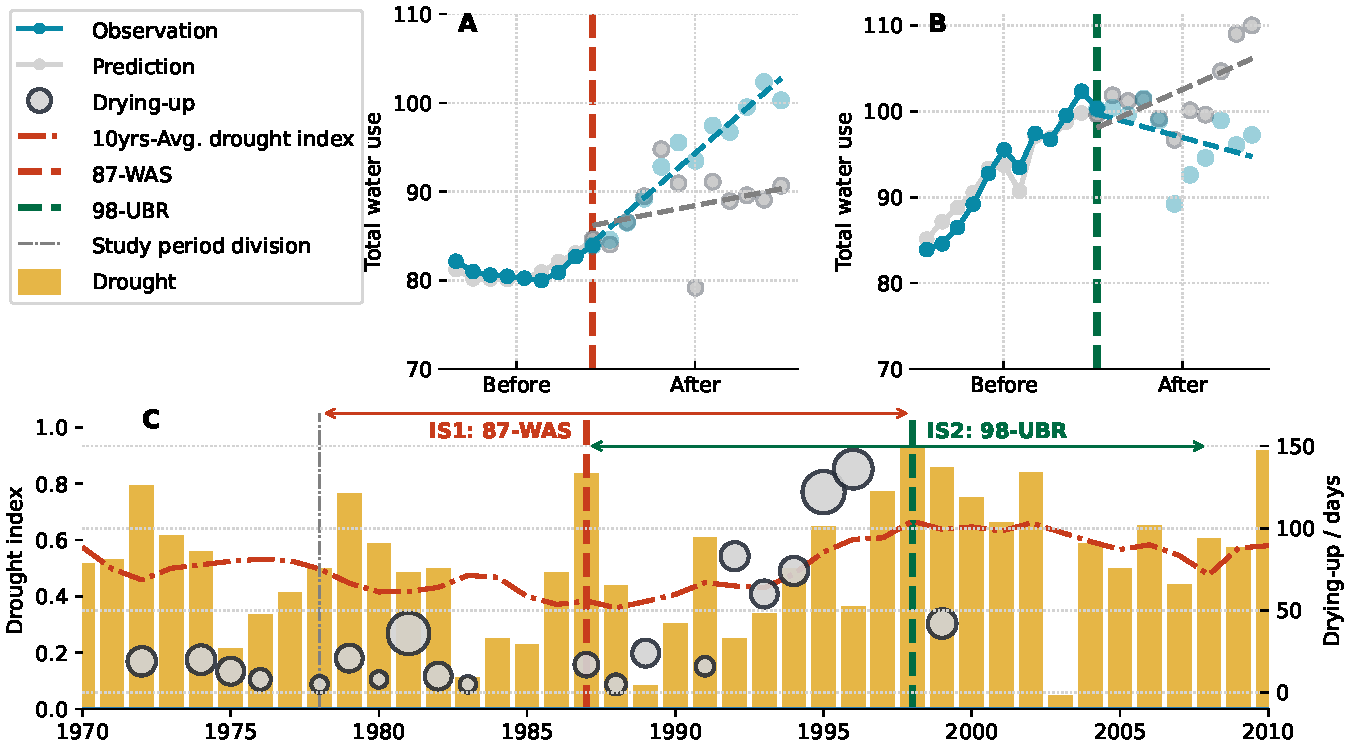
\includegraphics[width=\linewidth]{img/ch5/main_results2.pdf}
	\caption[两种制度变迁对黄河流域水资源利用与配置的影响]{
        两种制度变迁对黄河流域水资源利用与配置的影响
        \textbf{A.} “八七”分水方案前后黄河流域用水量;
        \textbf{B.} 流域统一调度前后黄河流域的用水情况。蓝线是来自统计资料的用水量,灰色线为经济和环境背景控制下差分综合控制法的估计值;
        \textbf{C.} 黄河流域干旱强度与断流事件,灰色气泡的大小表示断流河段的长度。
	}\label{fig:main_results}
\end{figure}

对用水量的理论估计表明,“八七”分水方案的制度转变促使各省取用了更多的水资源(图~\ref{fig:main_results}~A),1988年至1998年,反事实推断模型所估计的各省总用水量仅为$9743.4$亿立方米,但统计实际值达到了$10383.6$亿立方米(增加了$6.57\%$)。
在1998年流域统一调度制度出台后,用水量持续增加的趋势得到了抑制,从1998年到2008年,统计实际总用水量以每年$4.9$亿立方米的速度减少,而反事实推断所估计的用水量以$8.2$亿立方米每年的速度增加(图~\ref{fig:main_results}~B)。
“八七”分水方案后用水量的增加与$1987 \sim 1998$年日益严重的黄河断流相一致,无论是断流时长还是断流河段长度都在此时期内持续增加,导致流域生态退化和环境危机(图~\ref{fig:main_results}~C)。
尽管$1998 \sim 1987$年黄河流域的平均干旱强度还高于$1987 \sim 1998$年(平均干旱指数从“八七”分水方案后的$0.47$提升至流域统一调度后的$0.62$,图~\ref{fig:main_results}~C),1998年提出的流域统一调度却立竿见影地结束了长达二十余年的河流断流。

%\subsection{REGIONAL DIFFERENCES IN RESPONSES TO INSTITUTIONAL SHIFTS}
\subsection{对制度变化的响应差异}\label{result-3}

\begin{figure}[!htb]
	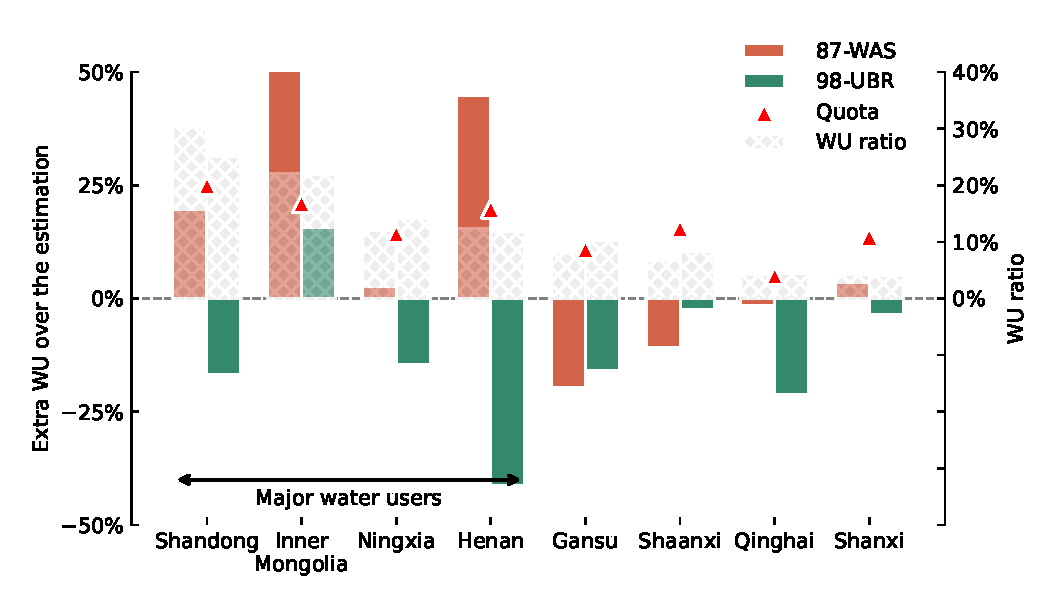
\includegraphics[width=\textwidth]{img/ch5/fig3.pdf}
	\caption[黄河流域各省份对制度变化的响应差异]{黄河流域各省份对制度变化的响应差异。红色柱状图(“八七”分水方案)和绿色柱状图(流域统一调度)分别表示在此次制度转变后的十年内,实际用水量相对于反事实推断模型估计值的增减比例。灰色柱状图显示了在两次制度转变后的十年那,各省实际用水量相对于其总用水量的比例。三角形标记指示“八七”分水方案为该省制定的理论水资源配额所占黄河流域总可用水量的比值。}\label{fig:regulating}
\end{figure}

% 结果2部分:展示区域相应差异
研究结果还表明各省(或地区)对这两次水资源分配制度改革(“八七”分水方案和流域统一调度)的响应模式存在差异。
在“八七”分水方案后的十年间,各省用水量相对反事实推断模型所估计用水量增加(或减少)的比例与其当前从黄河流域的取用水占比显著正相关(偏相关系数为$0.77$, $p<0.05$,图~\ref{fig:regulating})。
从1987年到1998年,一些用水大省(如内蒙古、河南、山东)也出现了显著的用水量增加(图~\ref{fig:regulating}),山东、内蒙古、河南和宁夏四省的用水量平均比预测值高出$32.14\%$。
而在施行流域统一调度后的1998年至2008年,几乎所有省份的用水量都出现了下降(平均下降$16.54\%$),
且各省用水量与从黄河流域的取用水占比不再呈相关性(偏相关系数为$0.33$, $p>0.1$)。
